% Provenance (never printed): see sources/outline_sources.md (Year 3:
% Darcy's law; permeability; aquifer types; the groundwater-flow equation;
% pumping tests; solute transport, in principle).
% Brief: sources/book5/BRIEFS.md, ch. 23. Curves from figdata/bachelor-3/
% theis.py, flow_net.py and advection_dispersion.py; the site of Varden-3 from
% figdata/shared/region.py (read only). Exercise and problem values in the
% Book 5 scratch calculator calc/ch23.py. The wells, the dam, the tests and
% the solutes are invented.
\chapter{Hidrogeologia}\label{ch:b3:hydrogeology}

Um poço novo bombeia \qty{2160}{m^3} de água por dia de um calcário a algumas
centenas de metros abaixo de uma fazenda. A princípio, nada acontece ao poço da
fazenda. Um mês depois, o nível da água nele está quase \qty{2}{m} mais baixo, embora
ele fique a um quilômetro de distância, e a estação de bombeamento nunca tenha retirado dele uma gota.
Ao redor do poço novo, o nível da água não caiu de modo uniforme: ele afundou formando um
\omterm{def:b3:hydrogeology:cone}{cone de depressão}, e o cone cresceu depressa através de uma rocha na qual a própria água
se move alguns centímetros por dia. Este capítulo constrói a física que
prevê os dois números: a propagação rápida da pressão e o deslocamento lento
da água, a partir de uma única lei empírica encontrada em 1856.
% ledger: heath:darcy

\begin{recall}
Porosidade, permeabilidade, nível freático, águas subterrâneas, aquíferos, nascentes
e poços estão nos volumes escolares, assim como o tempo de residência da água e
da água subterrânea fóssil. Viscosidade, a lei de Poiseuille para o escoamento em um tubo e a
equação de difusão estão nos volumes de física. A função erro
e as soluções da equação de difusão que a usam estão no
Capítulo~\ref{ch:b3:lithosphere-thermal-models}. Os Varden Hills, a
região inventada da série, com seus arenitos, calcários, folhelhos e giz, são
a região dos exercícios desde os volumes escolares.
\end{recall}

\section{Carga hidráulica e lei de Darcy}\label{sec:b3:hydrogeology:darcy}

A água subterrânea se move de onde sua energia mecânica por unidade de peso é
alta para onde é baixa. Como ela se move lentamente, sua energia cinética é
desprezível, e essa energia tem duas parcelas: a altura da água e sua
pressão.

\begin{definition}[Carga hidráulica; gradiente hidráulico]\label{def:b3:hydrogeology:head}
A \emph{carga hidráulica}\index{carga hidráulica} em um ponto do
solo saturado é
\[
h = z + \frac{p}{\rho g} ,
\]
a soma da \emph{carga de elevação} $z$ do ponto acima de um nível de referência e da
\emph{carga de pressão} $p/(\rho g)$, sendo $p$ a pressão da água acima da
pressão atmosférica. É a altura até a qual a água sobe em um
tubo, um piezômetro, aberto apenas nesse ponto. O \emph{gradiente
hidráulico}\index{gradiente hidráulico} é $\nabla h$; seu módulo entre dois
pontos separados por uma distância $L$ ao longo do escoamento é $\Delta h/L$.
\end{definition}

\begin{omfigure}
\centering
\begin{tikzpicture}[>=stealth, font=\small, x=1cm, y=1cm]
\fill[omLithAlluv!60] (0,-0.6) rectangle (7,3.2);
\fill[omSea!45] (0,-0.6) rectangle (7,1.9);
\draw[thick, brown!60!black] (0,3.2) -- (7,3.2);
\draw[omDef, dashed] (0,1.9) -- (7,1.9);
\node[omDef, font=\scriptsize, anchor=south east] at (6.9,1.92) {nível freático};
% piezometer
\fill[white] (3.3,0.4) rectangle (3.7,4.0);
\draw[thick] (3.3,0.7) -- (3.3,4.0); \draw[thick] (3.7,0.7) -- (3.7,4.0);
\draw[thick, densely dotted] (3.3,0.4) -- (3.3,0.7); \draw[thick, densely dotted] (3.7,0.4) -- (3.7,0.7);
\fill[omSea!70] (3.32,0.4) rectangle (3.68,2.6);
\draw[omDef, thick] (3.3,2.6) -- (3.7,2.6);
\fill (3.5,0.55) circle (0.06);
\node[font=\scriptsize, anchor=west] at (3.75,0.55) {filtro, no ponto $P$};
% datum
\draw[black!60] (0,-0.6) -- (7,-0.6);
\node[font=\scriptsize, anchor=north west] at (0,-0.62) {referência, $z = 0$};
% heads, on the left of the tube
\draw[<->] (2.5,-0.6) -- node[left, font=\scriptsize] {$z$} (2.5,0.55);
\draw[<->] (2.5,0.55) -- node[left, font=\scriptsize] {$p/\rho g$} (2.5,2.6);
\draw[black!40, densely dashed] (2.4,0.55) -- (3.3,0.55);
\draw[black!40, densely dashed] (1.0,2.6) -- (3.3,2.6);
\draw[<->, thick, omThm] (1.1,-0.6) -- node[left, font=\scriptsize] {$h$} (1.1,2.6);
\node[font=\scriptsize, anchor=south] at (3.5,4.0) {piezômetro};
\end{tikzpicture}

\par\smallskip{\small Um piezômetro, um tubo aberto apenas no seu filtro. A
água fica nele na \omterm{def:b3:hydrogeology:head}{carga hidráulica} do ponto $P$: sua elevação
$z$ mais sua carga de pressão. Aqui o nível no tubo está acima do nível
freático, como ocorre onde a água sobe em direção a uma nascente ou a um
rio.}\label{fig:b3:hydrogeology:head}
\end{omfigure}

Em 1856, Henry Darcy, engenheiro francês, mediu o escoamento de água através de
colunas de areia e constatou que ele era proporcional à perda de carga por unidade
de comprimento. O escoamento é laminar: a água segue linhas de corrente separadas.
% ledger: heath:darcy

\begin{theorem}[Lei de Darcy]\label{thm:b3:hydrogeology:darcy}
Em um meio poroso saturado, o volume de água que atravessa a área unitária por
unidade de tempo é
\[
\vec q = -K\,\nabla h ,
\]
em que $K$ depende do meio e do fluido. Em um meio cujos poros
são tubos retos paralelos de raio $a$ ocupando uma fração $n$ do
volume, a lei de Poiseuille fornece esta lei com
\[
K = \frac{k\rho g}{\mu}, \qquad k = \frac{na^2}{8} ,
\]
sendo $\mu$ a viscosidade da água.
\end{theorem}
\index{lei de Darcy}

\begin{proof}
A primeira afirmação é a lei empírica de Darcy. Em um tubo de raio $a$
ao longo do escoamento, a lei de Poiseuille fornece a velocidade média $\bar u =
-(a^2/8\mu)\,\mathrm d(p + \rho gz)/\mathrm dl = -(a^2\rho g/8\mu)\,\mathrm
dh/\mathrm dl$, já que $p + \rho gz = \rho g h$. Os tubos ocupam a
fração $n$ de qualquer seção transversal, logo o volume por unidade de área total é
$q = n\bar u = -(na^2/8)(\rho g/\mu)\,\mathrm dh/\mathrm dl$.
\end{proof}

Poros reais não são tubos retos; o teorema mostra a forma da lei
e como ela varia com a escala. O fluxo é proporcional ao gradiente, ao quadrado
do tamanho dos poros e inversamente proporcional à viscosidade: a mesma areia
deixa a água passar mais depressa quando ela está quente.

\begin{definition}[Vazão específica; condutividade hidráulica; permeabilidade intrínseca]\label{def:b3:hydrogeology:darcy}
A \emph{vazão específica}\index{vazão específica} $\vec q$ é o
volume de água que atravessa a unidade de área do meio, grãos e poros
em conjunto, por unidade de tempo. A \emph{condutividade
hidráulica}\index{condutividade hidráulica} $K$ é o coeficiente da
\omterm{thm:b3:hydrogeology:darcy}{lei de Darcy}, em \unit{m/s} ou \unit{m/d}. A \emph{permeabilidade
intrínseca}\index{permeabilidade intrínseca} do meio é $k =
K\mu/(\rho g)$, em \unit{m^2}: ela depende apenas do meio.
\end{definition}

A \omterm{def:b3:hydrogeology:darcy}{condutividade hidráulica} das rochas abrange doze ordens de
grandeza, como poucas grandezas físicas o fazem. Lendo-se o gráfico de um
levantamento clássico do assunto, os intervalos típicos, em metros por dia, são: argila
\num{e-7} a \num{e-4}; silte e loess \num{e-3} a 2; areia siltosa 0.04 a
10; areia limpa 0.3 a 150; cascalho 100 a 4000; folhelho \num{e-8} a
\num{e-4}; arenito \num{e-5} a 0.4; rochas carbonáticas \num{e-4} quando
são apenas fraturadas, até vários milhares quando são cavernosas; rochas ígneas e
metamórficas abaixo de \num{e-8} quando não fraturadas, até alguns quando
fraturadas. A maioria das rochas também conduz a água melhor ao longo do acamamento
do que transversalmente a ele.
% ledger: heath:darcy, heath:k-chart

A \omterm{def:b3:hydrogeology:darcy}{vazão específica} é um fluxo através de toda a área; a água escoa
apenas pelos poros, e com maior velocidade.

\begin{definition}[Velocidade de percolação]\label{def:b3:hydrogeology:seepage}
A \emph{velocidade de percolação}\index{velocidade de percolação} é $\vec v = \vec
q/n_e$, a velocidade média da água nos poros, sendo $n_e$ a
porosidade efetiva, isto é, a dos poros conectados pelos quais a água
escoa.
\end{definition}

Uma areia grossa com $K = \qty{60}{m/d}$, \omterm{def:b3:hydrogeology:head}{gradiente hidráulico} de 1 para 1000 e uma
porosidade de 0.20 move sua água a \qty{0.3}{m/d}; uma argila com $K =
\qty{e-4}{m/d}$, \omterm{def:b3:hydrogeology:head}{gradiente hidráulico} de 1 para 10 e porosidade de 0.50, a
\qty{2e-5}{m/d}, menos de um centímetro por ano. A água subterrânea não escoa
em rios subterrâneos, exceto nas cavernas de calcários e nos tubos de
lava. Esses são valores médios: onde um poluente se desloca, sua parte mais rápida pode
ir várias vezes mais depressa.
% ledger: heath:velocity

\section{Aquíferos}\label{sec:b3:hydrogeology:aquifers}

\begin{definition}[Aquíferos confinados e livres; aquitardo]\label{def:b3:hydrogeology:aquifer-types}
Um \emph{aquífero livre}\index{aquífero livre} é um aquífero cuja
superfície superior é o nível freático. Um \emph{aquífero
confinado}\index{aquífero confinado} é um aquífero sobreposto por uma camada de condutividade
muito menor, de modo que a água nele está sob pressão: num poço que o atinge, a água sobe
acima do topo do aquífero, até sua
superfície potenciométrica. Uma camada de baixa condutividade que retarda, mas não
interrompe a passagem de água entre aquíferos, é um
\emph{aquitardo}\index{aquitardo}.
\end{definition}

\begin{definition}[Transmissividade; coeficiente de armazenamento; rendimento específico]\label{def:b3:hydrogeology:storage}
A \emph{transmissividade}\index{transmissividade} de um aquífero de espessura
$b$ é $T = Kb$, a vazão por unidade de largura sob gradiente unitário, em
\unit{m^2/d}. Seu \emph{coeficiente de armazenamento}\index{coeficiente de armazenamento} $S$ é o
volume de água liberado por unidade de área do
aquífero quando a carga cai uma unidade; é adimensional. O
\emph{rendimento específico}\index{rendimento específico} $S_y$ de uma rocha é o volume
de água que drena dela por gravidade, por unidade de volume, quando o nível
freático desce através dela.
\end{definition}

Os dois tipos de aquífero liberam água de maneiras diferentes. Em um \omterm{def:b3:hydrogeology:aquifer-types}{aquífero confinado}
a carga cai, mas os poros continuam cheios: a água se expande um
pouco, e o aquífero, suportando mais do peso das rochas sobrejacentes,
se comprime um pouco. A expansão da água, sozinha, libera cerca de
\num{9e-7} metro cúbico por metro cúbico de aquífero e por metro de carga;
com a compressão, o \omterm{def:b3:hydrogeology:storage}{coeficiente de armazenamento} da maioria dos \omterm{def:b3:hydrogeology:aquifer-types}{aquíferos confinados} é
\num{e-5} a \num{e-3}. Em um \omterm{def:b3:hydrogeology:aquifer-types}{aquífero livre} o nível freático desce e
os poros acima dele drenam: o \omterm{def:b3:hydrogeology:storage}{coeficiente de armazenamento} é o \omterm{def:b3:hydrogeology:storage}{rendimento específico}, cerca de 0.1
a 0.3, de cem a dez mil vezes maior. As \omterm{def:b3:hydrogeology:storage}{transmissividades} dos
aquíferos em uso variam de menos de \qty{1}{m^2/d} em rochas fraturadas
a \qty{100000}{m^2/d} em calcários cavernosos e derrames de lava. Quando a
carga de um \omterm{def:b3:hydrogeology:aquifer-types}{aquífero confinado} é rebaixada por longo tempo, as argilas dentro e
em torno dele drenam e se compactam, e o terreno acima sofre subsidência.
% ledger: heath:storage, heath:transmissivity

\begin{omfigure}
\centering
\begin{tikzpicture}[>=stealth, font=\small, x=1cm, y=1.1cm]
\begin{scope}
\clip (0,-1.3) -- (0,2.0) -- (3.5,2.9) -- (5,3.5) -- (7.5,4.2) -- (11,3.8) -- (11,-1.3) -- cycle;
\fill[lith sandstone] (0,-1.3) rectangle (11,4.5);
\fill[lith limestone] (0,1.8) -- (11,-0.95) -- (11,0.05) -- (0,2.8) -- cycle;
\fill[lith shale] (0,2.8) -- (11,0.05) -- (11,1.25) -- (0,4.0) -- cycle;
\fill[omLithLime!25] (0,4.0) -- (11,1.25) -- (11,4.5) -- (0,4.5) -- cycle;
\end{scope}
\draw[thick, brown!60!black] (0,2.0) -- (3.5,2.9) -- (5,3.5) -- (7.5,4.2) -- (11,3.8);
% water table in the chalk
\draw[omDef, dashed, thick] (4.5,3.0) .. controls (6,3.35) and (8.5,3.35) .. (11,2.8);
\node[omDef, font=\scriptsize, anchor=south] at (6.6,3.32) {nível freático};
% potentiometric surface of the limestone
\draw[omThm, densely dashdotted, thick] (1.4,2.36) -- (11,2.2);
\node[omThm, font=\scriptsize, anchor=south east, fill=white, inner sep=1pt] at (10.9,2.25) {superfície potenciométrica do calcário};
% well Varden-3
\draw[thick] (2.9,2.74) -- (2.9,1.05); \draw[thick] (3.1,2.8) -- (3.1,1.05);
\fill[omDef!35] (2.92,1.05) rectangle (3.08,2.33);
\draw[omThm, thick] (2.85,2.33) -- (3.15,2.33);
\node[font=\scriptsize, anchor=south] at (3.0,2.95) {Varden-3};
% labels
\node[font=\scriptsize, fill=white, inner sep=1pt] at (7.5,0.45) {calcário: aquífero confinado};
\node[font=\scriptsize, fill=white, inner sep=1pt] at (7.5,1.5) {folhelho: camada confinante};
\node[font=\scriptsize, fill=white, inner sep=1pt] at (8.4,2.8) {giz: aquífero livre};
\node[font=\scriptsize, fill=white, inner sep=1pt] at (7.5,-0.8) {arenito};
\node[font=\scriptsize, fill=white, inner sep=1pt, align=center] at (0.8,1.75) {calcário\\afloramento};
\draw[->, omDef, thick] (0.8,3.0) -- (0.8,2.3);
\node[omDef, font=\scriptsize, anchor=south] at (0.8,3.0) {recarga};
\end{tikzpicture}

\par\smallskip{\small Um corte esquemático da cobertura das Varden Hills
de O para L, fora de escala. O giz contém um \omterm{def:b3:hydrogeology:aquifer-types}{aquífero livre}
abaixo do seu nível freático. O calcário jurássico é recarregado onde aflora
e é confinado sob o folhelho: no poço Varden-3 do
problema, perfurado através do folhelho e aberto apenas ao calcário, a
água sobe até a superfície potenciométrica, muito acima do topo do
aquífero, mas abaixo do terreno.}\label{fig:b3:hydrogeology:aquifers}
\end{omfigure}
% ledger: region:name

\section{A equação do fluxo de águas subterrâneas}\label{sec:b3:hydrogeology:flow-equation}

\begin{theorem}[Equação do fluxo de águas subterrâneas]\label{thm:b3:hydrogeology:flow-equation}
Em um \omterm{def:b3:hydrogeology:aquifer-types}{aquífero confinado}, com \omterm{def:b3:hydrogeology:storage}{transmissividade} $T$ e \omterm{def:b3:hydrogeology:storage}{coeficiente de armazenamento} $S$ constantes,
com escoamento horizontal, a \omterm{def:b3:hydrogeology:head}{carga hidráulica} $h(x, y, t)$ obedece
\[
S\,\frac{\partial h}{\partial t} = T\nabla^2h + W ,
\]
sendo $W$ o volume de água acrescentado por unidade de área e de tempo pela recarga ou
retirado por bombeamento (negativo). Em escoamento estacionário sem fontes, $\nabla^2h =
0$.
\end{theorem}
\index{equação do fluxo de águas subterrâneas}

\begin{proof}
Considera-se uma coluna do aquífero de área $\mathrm dx\,\mathrm dy$. O fluxo por
unidade de largura através de toda a sua espessura é $-T\nabla h$, pela \omterm{thm:b3:hydrogeology:darcy}{lei de Darcy}
vezes $b$. A entrada líquida é $-\nabla\cdot(-T\nabla h)\,\mathrm dx\,\mathrm
dy = T\nabla^2h\,\mathrm dx\,\mathrm dy$. A água armazenada na coluna
varia à taxa $S\,(\partial h/\partial t)\,\mathrm dx\,\mathrm dy$,
pela definição de $S$. A conservação de massa, com a densidade da água
tratada como constante no balanço, iguala o armazenamento à entrada somada às fontes.
\end{proof}

É a equação de difusão dos volumes de física, com a difusividade
hidráulica $T/S$ no lugar de uma térmica. Para um calcário confinado com
$T = \qty{450}{m^2/d}$ e $S = \num{2e-4}$, a difusividade é
\qty{2.25e6}{m^2/d}: uma variação de carga se propaga por \qty{1}{km} em
cerca de $L^2S/T$, meio dia. O mesmo calcário, livre, com $S =
0.2$, levaria mil vezes mais tempo. A pressão se propaga rapidamente, a
água se move lentamente: os dois números da abertura.

\begin{proposition}[Escoamento radial estacionário para um poço]\label{prop:b3:hydrogeology:thiem}
Um poço bombeia $Q$ de um \omterm{def:b3:hydrogeology:aquifer-types}{aquífero confinado} de \omterm{def:b3:hydrogeology:storage}{transmissividade} $T$, sendo o
escoamento estacionário e radial. Entre duas distâncias $r_1 < r_2$ do poço, os
rebaixamentos diferem de
\[
s_1 - s_2 = \frac{Q}{2\pi T}\ln\frac{r_2}{r_1} .
\]
\end{proposition}

\begin{proof}
Através de todo círculo de raio $r$ em torno do poço, a vazão de entrada é $Q = 2\pi r
T\,\mathrm dh/\mathrm dr$. Integrando $\mathrm dh = (Q/2\pi T)\,\mathrm
dr/r$ de $r_1$ a $r_2$ e escrevendo $s = h_0 - h$, obtém-se o resultado.
\end{proof}

Em duas dimensões, desenha-se o escoamento estacionário com uma \omterm{def:b3:hydrogeology:flow-net}{rede de fluxo}.

\begin{definition}[Rede de fluxo]\label{def:b3:hydrogeology:flow-net}
Uma \emph{rede de fluxo}\index{rede de fluxo} é um desenho do escoamento estacionário de água subterrânea em
um corte homogêneo e isótropo por duas famílias de curvas: equipotenciais,
linhas de mesma carga, e linhas de corrente, que a água segue. As
linhas de corrente cruzam as equipotenciais em ângulo reto, e em uma rede de fluxo
são espaçadas de modo que as células sejam quadrados curvilíneos.
\end{definition}

\begin{method}[Percolação a partir de uma rede de fluxo]\label{met:b3:hydrogeology:flow-net}
\leavevmode
\begin{enumerate}
\item Desenham-se os contornos: um contorno impermeável é uma linha de corrente; o leito de um
  corpo de água, onde a carga é fixa, é uma equipotencial.
\item Desenham-se $N_d$ quedas de carga entre as cargas mais alta e mais baixa, $\Delta h
  = H/N_d$, e as linhas de corrente formando $N_f$ canais de fluxo, por tentativa,
  até que cada célula seja um quadrado curvilíneo.
\item Cada canal transporta $K\Delta h$ por unidade de comprimento normal ao
  corte, cancelando-se o comprimento e a largura do quadrado: o total é $q =
  KHN_f/N_d$.
\end{enumerate}
\end{method}

\begin{omfigure}
\centering
\begin{tikzpicture}
\begin{axis}[width=0.95\linewidth, height=0.36\linewidth, axis equal image,
  xmin=-60, xmax=60, ymin=-20, ymax=13, xlabel={$x$ (\unit{m})}, ylabel={$z$ (\unit{m})},
  tick label style={font=\scriptsize}, label style={font=\small}, clip=false]
% computed in figdata/bachelor-3/flow_net.py
\fill[omLithAlluv!35] (axis cs:-60,-20) rectangle (axis cs:60,0);
\fill[omSea!40] (axis cs:-60,0) rectangle (axis cs:-10,11.2);
\fill[omSea!40] (axis cs:10,0) rectangle (axis cs:60,1.2);
\fill[black!35] (axis cs:-10,0) -- (axis cs:-10,12.5) -- (axis cs:-5,12.5) -- (axis cs:10,0) -- cycle;
\pgfplotsinvokeforeach{1,...,9}{
  \addplot[omThm, thin, unbounded coords=jump] table[x=x, y=z] {figdata/out/bachelor-3-flow_net-h-#1.dat};}
\pgfplotsinvokeforeach{1,...,4}{
  \addplot[omMeth, thick, unbounded coords=jump] table[x=x, y=z] {figdata/out/bachelor-3-flow_net-psi-#1.dat};}
\draw[very thick] (axis cs:-60,-20) -- (axis cs:60,-20);
\node[font=\scriptsize, anchor=south] at (axis cs:45,-19.6) {rocha impermeável};
\node[font=\scriptsize, align=center] at (axis cs:-36,6) {reservatório, \qty{10}{m} acima\\da água de jusante};
\node[font=\scriptsize, anchor=south] at (axis cs:35,1.4) {água de jusante};
\node[font=\scriptsize] at (axis cs:-4,4) {barragem};
\end{axis}
\end{tikzpicture}

\par\smallskip{\small Percolação sob uma barragem de \qty{20}{m} de largura sobre uma camada de
areia com \qty{20}{m} de espessura, o reservatório \qty{10}{m} acima da água
de jusante, calculada resolvendo a equação de Laplace para a carga e para a
função de corrente. Linhas finas: equipotenciais, uma a cada metro de carga.
Linhas grossas: quatro linhas de corrente que, junto com a base da barragem e o fundo,
delimitam cinco canais de fluxo. A percolação calculada é $0.51\,KH$ por metro de
barragem; a \omterm{def:b3:hydrogeology:flow-net}{rede de fluxo} fornece $KH \times 5/10 = 0.50\,KH$.}\label{fig:b3:hydrogeology:flow-net}
\end{omfigure}

\section{Testes de bombeamento}\label{sec:b3:hydrogeology:pumping}

O fluxo estacionário para um poço é raro: um novo estado estacionário pode levar meses ou
anos, ou nunca se estabelecer. Em 1935, Theis, do Serviço Geológico
dos Estados Unidos, forneceu o rebaixamento ao redor de um poço bombeado a uma vazão constante, como
função do tempo, a partir da qual um teste de algumas horas ou dias fornece a
\omterm{def:b3:hydrogeology:storage}{transmissividade} e o \omterm{def:b3:hydrogeology:storage}{coeficiente de armazenamento} do aquífero.
% ledger: heath:theis

\begin{theorem}[Solução de Theis]\label{thm:b3:hydrogeology:theis}
Um poço que penetra totalmente um \omterm{def:b3:hydrogeology:aquifer-types}{aquífero confinado}, infinito e homogêneo, de
\omterm{def:b3:hydrogeology:storage}{transmissividade} $T$ e \omterm{def:b3:hydrogeology:storage}{coeficiente de armazenamento} $S$, começa a bombear em $t = 0$ a
vazão constante $Q$. O rebaixamento à distância $r$ é
\[
s(r, t) = \frac{Q}{4\pi T}\,W(u), \qquad u = \frac{r^2S}{4Tt}, \qquad
W(u) = \int_u^\infty\frac{\mathrm e^{-y}}{y}\,\mathrm dy = -\gamma - \ln u +
u - \frac{u^2}{2\cdot2!} + \frac{u^3}{3\cdot3!} - \cdots,
\]
com $\gamma = \num{0.5772}$. $W$ é denominada função do poço.
\end{theorem}
\index{Solução de Theis}

\begin{proof}
Na forma radial, a equação de fluxo é $S\,\partial s/\partial t =
T\,r^{-1}\partial_r(r\,\partial_rs)$, com $s = 0$ em $t = 0$, $s \to 0$ quando
$r \to \infty$ e $2\pi rT\,\partial_rs \to -Q$ quando $r \to 0$. Nenhum dos
dados contém um comprimento ou um tempo isoladamente, então tenta-se $s = f(u)$ com $u =
r^2S/4Tt$. Como $\partial_ru = 2u/r$ e $\partial_tu = -u/t$, tem-se $r\,\partial_rs =
2uf'$, $r^{-1}\partial_r(r\,\partial_rs) = (4u/r^2)(uf')'$ e $\partial_ts =
-(u/t)f'$. Multiplicando a equação por $r^2/(4Tu)$ resulta $(uf')' = -uf'$:
com $g = uf'$, tem-se $g' = -g$ e $g = c\,\mathrm e^{-u}$. A condição do poço, $2\pi T\cdot2uf' \to -Q$ quando $u \to 0$, dá $c =
-Q/4\pi T$, e $f(\infty) = 0$ dá $f(u) = (Q/4\pi T)\int_u^\infty
\mathrm e^{-y}y^{-1}\,\mathrm dy$. A série segue de
$W(u) = -\gamma - \ln u + \int_0^u(1 - \mathrm e^{-y})\,y^{-1}\,\mathrm dy$,
com a constante sendo a de Euler, integrando termo a termo.
\end{proof}

\begin{proposition}[Aproximação de Cooper--Jacob]\label{prop:b3:hydrogeology:cooper-jacob}
Quando $u \le 0.05$, o rebaixamento de Theis fica próximo de
\[
s = \frac{2.3\,Q}{4\pi T}\log_{10}\frac{2.25\,Tt}{r^2S} :
\]
plotado contra $\log_{10}t$, o rebaixamento é uma reta cujo aumento por
ciclo logarítmico, $\Delta s$, fornece $T = 2.3\,Q/(4\pi\Delta s)$, e cujo
intercepto com $s = 0$, em $t_0$, fornece $S = 2.25\,Tt_0/r^2$.
\end{proposition}
\index{Aproximação de Cooper--Jacob}

\begin{proof}
Para $u$ pequeno, a série é $W \approx -\gamma - \ln u = \ln(\mathrm
e^{-\gamma}/u) = \ln(0.5615\cdot4Tt/r^2S) = \ln(2.25\,Tt/r^2S)$; o próximo
termo, $u$, é no máximo \num{0.05}, abaixo de \qty{2}{\percent} de $W$ ali.
Como $\ln x = 2.3\log_{10}x$, o rebaixamento sobe $2.3\,Q/4\pi T$ por
fator de dez no tempo, e se anula quando $2.25\,Tt_0 = r^2S$.
\end{proof}

\begin{omfigure}
\begin{tikzpicture}
\begin{groupplot}[group style={group size=2 by 1, horizontal sep=1.5cm},
  width=0.48\linewidth, height=0.4\linewidth,
  tick label style={font=\scriptsize}, label style={font=\small}, title style={font=\small}]
\nextgroupplot[xmode=log, xlabel={$1/u$}, ylabel={$W(u)$}, xmin=0.1, xmax=1e4, ymin=0, ymax=9,
  title={a função do poço},
  legend style={font=\scriptsize, at={(0.03,0.97)}, anchor=north west}]
% computed in figdata/bachelor-3/theis.py
\addplot[omDef, thick] table[x=invu, y=W] {figdata/out/bachelor-3-theis-wu.dat};
\addlegendentry{Theis $W(u)$}
\addplot[omThm, densely dashed, thick] table[x=invu, y=Wcj] {figdata/out/bachelor-3-theis-cj.dat};
\addlegendentry{$-\gamma - \ln u$}
\addplot[black!40, densely dotted, forget plot] coordinates {(20,0) (20,9)};
\node[font=\scriptsize, black!60, anchor=west] at (axis cs:24,0.6) {$u = 0.05$};
\nextgroupplot[xmode=log, xlabel={tempo desde o início do bombeamento (\unit{min})}, ylabel={rebaixamento (\unit{m})},
  xmin=0.5, xmax=5000, ymin=0, ymax=3.4, title={Varden-3, $r = \qty{60}{m}$},
  legend style={font=\scriptsize, at={(0.03,0.97)}, anchor=north west}]
\addplot[only marks, mark=*, mark size=1.3pt] table[x=tmin, y=s] {figdata/out/bachelor-3-theis-test.dat};
\addlegendentry{medido}
\addplot[omMeth, thick, domain=0.973:5000, samples=2] {0.87221*log10(x/0.973132)};
\addlegendentry{reta de Cooper--Jacob}
\addplot[black!40, densely dotted, forget plot] coordinates {(11.5,0) (11.5,3.4)};
\end{groupplot}
\end{tikzpicture}

\par\smallskip{\small À esquerda, a função do poço de Theis contra $1/u$ em um
eixo logarítmico, e sua aproximação em reta: elas coincidem quando $u <
0.05$ (pontilhado). À direita, o rebaixamento registrado no poço de observação do
teste Varden-3 do problema, a \qty{60}{m} do poço bombeado, e a
reta ajustada aos pontos após \qty{11.5}{min}, onde $u <
0.05$: sua inclinação fornece $T$, seu intercepto, $S$.}\label{fig:b3:hydrogeology:theis}
\end{omfigure}
% ledger: heath:theis, heath:jacob

\begin{definition}[Cone de depressão]\label{def:b3:hydrogeology:cone}
O \emph{cone de depressão}\index{cone de depressão} de um poço bombeado é
o rebaixamento do nível freático, ou da superfície potenciométrica,
ao redor do poço; o gradiente se acentua em direção a ele, por onde toda
a água deve passar.
\end{definition}

Como os rebaixamentos obedecem a uma equação linear, os cones de vários poços
se somam. Em um \omterm{def:b3:hydrogeology:aquifer-types}{aquífero confinado}, com seu pequeno \omterm{def:b3:hydrogeology:storage}{coeficiente de armazenamento}, um cone cresce rapidamente
e os cones de poços vizinhos logo interferem; em um \omterm{def:b3:hydrogeology:aquifer-types}{aquífero livre},
que precisa drenar seus poros, o cone cresce lentamente. O cone para de crescer
só quando tiver captado recarga suficiente, ou reduzido o bastante
a descarga natural do aquífero para rios e nascentes, para equilibrar
o bombeamento. Grandes retiradas de um \omterm{def:b3:hydrogeology:aquifer-types}{aquífero confinado} alcançam longe: em 1981
cerca de \qty{277000}{m^3/d} bombeados do aquífero Cretáceo da planície costeira
atlântica, na Virgínia e na Carolina do Norte, haviam produzido
cones sobrepostos por toda a sua extensão.
% ledger: heath:cone

\begin{omfigure}
\begin{tikzpicture}
\begin{groupplot}[group style={group size=2 by 1, horizontal sep=1.5cm},
  width=0.48\linewidth, height=0.4\linewidth, y dir=reverse,
  tick label style={font=\scriptsize}, label style={font=\small}, title style={font=\small}]
\nextgroupplot[xlabel={distância do poço (\unit{m})}, ylabel={rebaixamento (\unit{m})},
  xmin=0, xmax=3000, ymin=0, ymax=6, title={o cone de um poço},
  scaled x ticks=false, xticklabel style={/pgf/number format/1000 sep={}},
  legend style={font=\scriptsize, at={(0.97,0.03)}, anchor=south east}]
% computed in figdata/bachelor-3/theis.py
\addplot[omThm!50, thick] table[x=r, y=s] {figdata/out/bachelor-3-theis-cone-1.dat};
\addlegendentry{1 dia}
\addplot[omThm!80, thick] table[x=r, y=s] {figdata/out/bachelor-3-theis-cone-10.dat};
\addlegendentry{10 dias}
\addplot[omThm!60!black, thick] table[x=r, y=s] {figdata/out/bachelor-3-theis-cone-100.dat};
\addlegendentry{100 dias}
\nextgroupplot[xlabel={$x$ (\unit{m})}, ylabel={rebaixamento (\unit{m})},
  xmin=-1500, xmax=1900, ymin=0, ymax=9, title={dois poços, 10 dias},
  scaled x ticks=false, xticklabel style={/pgf/number format/1000 sep={}},
  legend columns=3, legend style={font=\scriptsize, at={(0.5,0.985)}, anchor=north,
  /tikz/every even column/.append style={column sep=3pt}}]
\addplot[omDef, densely dashed] table[x=x, y=s1] {figdata/out/bachelor-3-theis-interf.dat};
\addlegendentry{poço em 0}
\addplot[omMeth, densely dashed] table[x=x, y=s2] {figdata/out/bachelor-3-theis-interf.dat};
\addlegendentry{poço em 400 m}
\addplot[black, thick] table[x=x, y=stot] {figdata/out/bachelor-3-theis-interf.dat};
\addlegendentry{ambos}
\end{groupplot}
\end{tikzpicture}

\par\smallskip{\small O cone de Theis do poço Varden-3 ($Q =
\qty{2160}{m^3/d}$, $T = \qty{450}{m^2/d}$, $S = \num{2e-4}$), com o rebaixamento
representado para baixo. À esquerda, após 1, 10 e 100 dias: o cone se aprofunda
da mesma quantidade a cada aumento de dez vezes no tempo e se alarga sem limite
em um aquífero infinito. À direita, dois desses poços separados por \qty{400}{m},
após 10 dias: os rebaixamentos se somam, com \qty{5.5}{m} no ponto médio entre
eles, em vez de \qty{2.7}{m} para um único poço.}\label{fig:b3:hydrogeology:cone}
\end{omfigure}
% ledger: heath:cone, heath:storage

\begin{inthefield}[Um teste de bombeamento]
\begin{minipage}[t]{0.55\linewidth}\vspace{0pt}
Antes de um teste de bombeamento, os hidrogeólogos registram os níveis de água nos
poços por algum tempo, para conhecer a tendência sobre a qual o teste será
superposto. A bomba então funciona com vazão constante, mantida estável e medida
por um medidor instalado no tubo de descarga, durante várias horas a vários dias.
Em cada poço de observação, pelo menos três deles, a distâncias diferentes se
possível, lê-se a profundidade da água abaixo de um ponto fixo de medição em
tempos conhecidos com precisão, muitas leituras nos primeiros minutos e menos depois, com
uma trena de aço graduada ou uma sonda elétrica cujo eletrodo fecha um circuito
ao tocar a água. Hoje, um transdutor de pressão submersível suspenso no
poço e ligado a um registrador eletrônico, registra o nível quase
continuamente.
\end{minipage}\hfill
\begin{minipage}[t]{0.42\linewidth}\vspace{0pt}
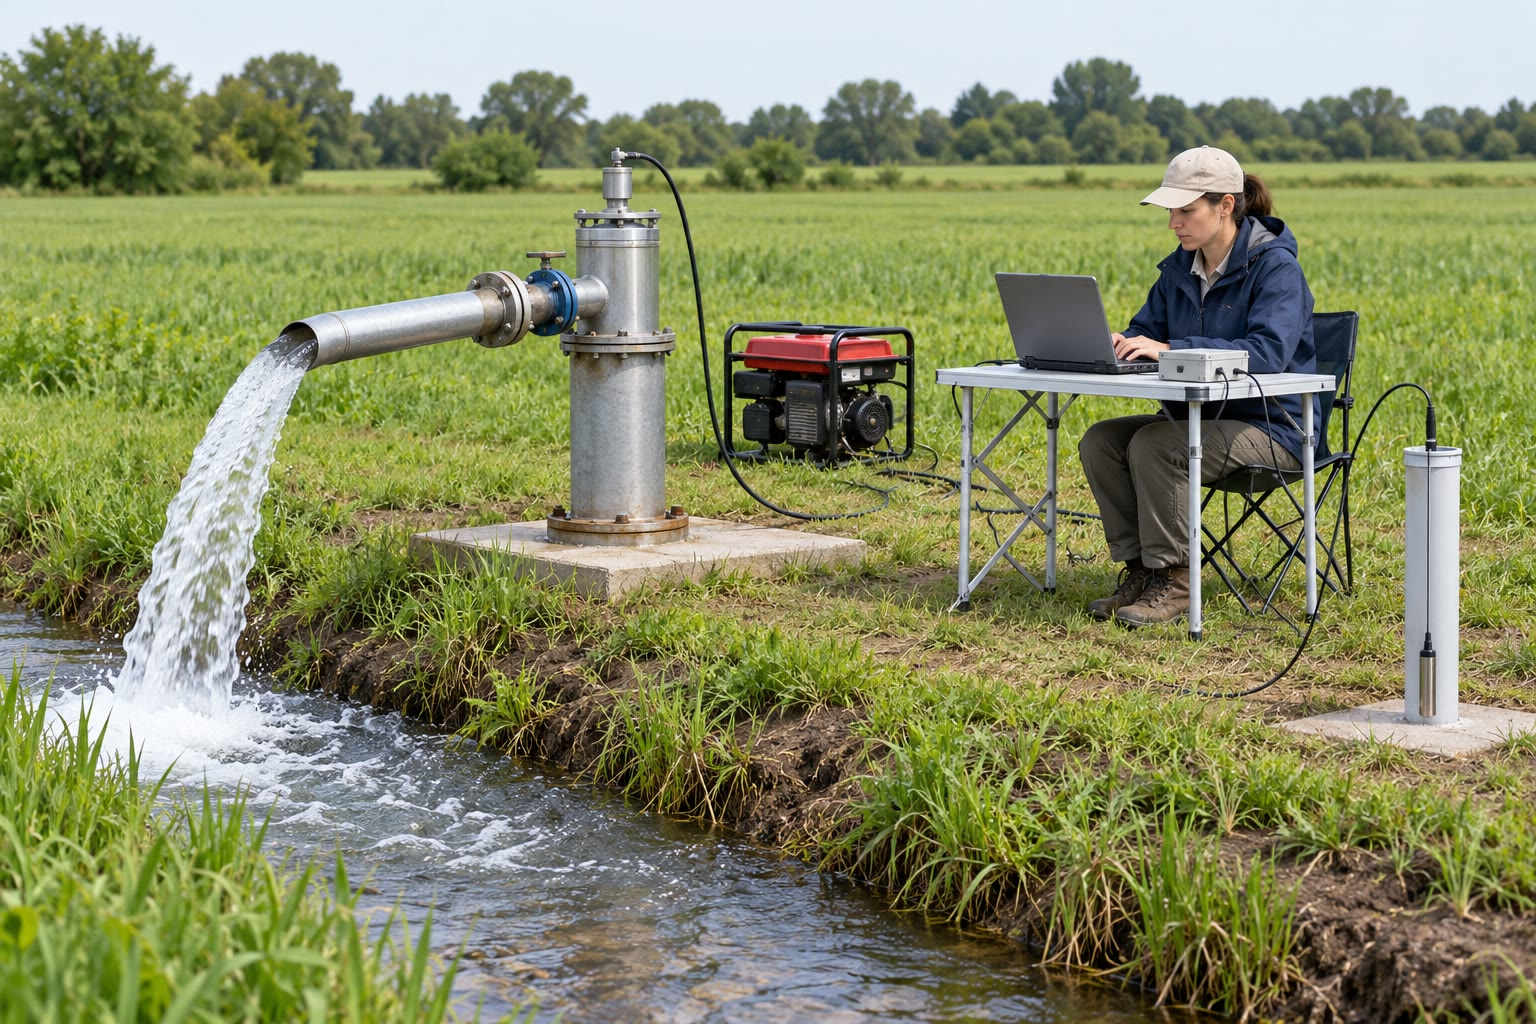
\includegraphics[width=\linewidth]{images/book5/ai/b3-pumping-test.jpg}

{\scriptsize Um teste de bombeamento: o tubo de descarga do poço bombeado, um
gerador e um hidrogeólogo registrando os níveis de um poço de observação
em um notebook (Ilustração gerada por IA.)}
\end{minipage}
\end{inthefield}
% ledger: heath:theis, heath:jacob, heath:water-levels, usgs:transducers

\section{Transporte de soluto}\label{sec:b3:hydrogeology:transport}

Um soluto dissolvido na água subterrânea é transportado com a água, na
\omterm{def:b3:hydrogeology:seepage}{velocidade de percolação}, e se espalha ao longo do caminho: a água nos poros vizinhos
se move em velocidades e por trajetos diferentes, e o soluto
também se difunde.

\begin{definition}[Dispersão hidrodinâmica; dispersividade]\label{def:b3:hydrogeology:ade}
A \emph{dispersão hidrodinâmica}\index{dispersão hidrodinâmica} é o
espalhamento de um soluto na água subterrânea em movimento, causado pelas variações da
velocidade da água de poro a poro e pela difusão molecular. Ao longo
do escoamento, ela é descrita por um coeficiente de dispersão $D = \alpha_Lv + D^*$,
em que $v$ é a \omterm{def:b3:hydrogeology:seepage}{velocidade de percolação}, $D^*$ é a difusividade molecular efetiva e
$\alpha_L$, um comprimento, é a
\emph{dispersividade}\index{dispersividade} longitudinal do meio.
\end{definition}

\begin{theorem}[Equação de advecção--dispersão]\label{thm:b3:hydrogeology:ade}
Ao longo de um escoamento unidimensional de \omterm{def:b3:hydrogeology:seepage}{velocidade de percolação} constante $v$, a
concentração $C(x, t)$ de um soluto não reativo obedece a
\[
\frac{\partial C}{\partial t} = D\,\frac{\partial^2C}{\partial x^2} -
v\,\frac{\partial C}{\partial x} .
\]
Se a concentração é mantida em $C_0$ em $x = 0$ a partir de $t = 0$, em um meio
inicialmente livre de soluto,
\[
\frac{C}{C_0} = \frac12\left[\operatorname{erfc}\frac{x - vt}{2\sqrt{Dt}} +
\mathrm e^{vx/D}\operatorname{erfc}\frac{x + vt}{2\sqrt{Dt}}\right] .
\]
\end{theorem}
\index{equação de advecção--dispersão}

\begin{proof}
Em uma fatia de seção transversal unitária e comprimento $\mathrm dx$, de porosidade
efetiva $n_e$, o soluto armazenado é $n_eC\,\mathrm dx$. Seu fluxo é
$n_e(vC - D\,\partial C/\partial x)$, transportado com a água e espalhado pela
dispersão, assim como a lei de Fick espalha uma substância que se difunde. A conservação dá
$n_e\partial_tC = -\partial_x[n_e(vC - D\partial_xC)]$, a equação. Que
a fórmula a satisfaz e às condições é admitido aqui;
O \cref{exo:b3:hydrogeology:12} verifica seu espalhamento.
\end{proof}

No referencial que se move com a água, $\xi = x - vt$, a equação é a
equação da difusão, e a frente se espalha como $\sqrt{2Dt} = \sqrt{2\alpha_L
vt} = \sqrt{2\alpha_Lx}$: a largura da frente cresce com a raiz quadrada da
distância percorrida.

\begin{definition}[Fator de retardo]\label{def:b3:hydrogeology:retardation}
Um soluto adsorvido nos grãos, em equilíbrio e em proporção à sua
concentração, desloca-se mais lentamente que a água. Seu
\emph{fator de retardo}\index{fator de retardo (sorção)} é
\[
R = 1 + \frac{\rho_bK_d}{n} ,
\]
$\rho_b$ sendo a densidade aparente seca do meio, $n$ sua porosidade e
$K_d$ o coeficiente de distribuição, a massa adsorvida por unidade de massa de
sólido dividida pela concentração na água. O soluto se move com $v/R$
e se dispersa com $D/R$.
\end{definition}

\begin{omfigure}
\begin{tikzpicture}
\begin{groupplot}[group style={group size=2 by 1, horizontal sep=1.5cm},
  width=0.48\linewidth, height=0.4\linewidth,
  tick label style={font=\scriptsize}, label style={font=\small}, title style={font=\small}]
\nextgroupplot[xlabel={tempo (dias)}, ylabel={$C/C_0$ a \qty{100}{m}},
  xmin=0, xmax=1000, ymin=0, ymax=1.05, title={curvas de ruptura},
  legend style={font=\scriptsize, at={(0.97,0.03)}, anchor=south east}]
% computed in figdata/bachelor-3/advection_dispersion.py
\addplot[omDef, thick] table[x=t, y=c1] {figdata/out/bachelor-3-advection_dispersion-btc.dat};
\addlegendentry{$\alpha_L = \qty{1}{m}$}
\addplot[omMeth, thick] table[x=t, y=c3] {figdata/out/bachelor-3-advection_dispersion-btc.dat};
\addlegendentry{$\alpha_L = \qty{3}{m}$}
\addplot[omThm, thick] table[x=t, y=c10] {figdata/out/bachelor-3-advection_dispersion-btc.dat};
\addlegendentry{$\alpha_L = \qty{10}{m}$}
\addplot[black, thick, densely dashed, forget plot] table[x=t, y=cR] {figdata/out/bachelor-3-advection_dispersion-btc.dat};
\node[font=\scriptsize, anchor=west, align=left] at (axis cs:640,0.45) {$\alpha_L = \qty{3}{m}$,\\ $R = 3$};
\addplot[black!40, densely dotted, forget plot] coordinates {(200,0) (200,1.05)};
\nextgroupplot[xlabel={distância (\unit{m})}, ylabel={$C/C_0$ após 150 dias},
  xmin=0, xmax=160, ymin=0, ymax=1.05, title={perfis},
  legend style={font=\scriptsize, at={(0.03,0.03)}, anchor=south west}]
\addplot[omDef, thick] table[x=x, y=c1] {figdata/out/bachelor-3-advection_dispersion-profile.dat};
\addlegendentry{$\alpha_L = \qty{1}{m}$}
\addplot[omMeth, thick] table[x=x, y=c3] {figdata/out/bachelor-3-advection_dispersion-profile.dat};
\addlegendentry{$\alpha_L = \qty{3}{m}$}
\addplot[omThm, thick] table[x=x, y=c10] {figdata/out/bachelor-3-advection_dispersion-profile.dat};
\addlegendentry{$\alpha_L = \qty{10}{m}$}
\addplot[black!40, densely dotted, forget plot] coordinates {(75,0) (75,1.05)};
\end{groupplot}
\end{tikzpicture}

\par\smallskip{\small Um soluto injetado continuamente em $x = 0$ em um
escoamento de \omterm{def:b3:hydrogeology:seepage}{velocidade de percolação} \qty{0.5}{m/d}. À esquerda, a concentração
a \qty{100}{m} a jusante em função do tempo: a própria água chega após
200 dias (pontilhado); quanto maior a \omterm{def:b3:hydrogeology:ade}{dispersividade}, mais cedo surgem os primeiros
traços e mais tarde se atinge a concentração plena. Um soluto adsorvido com $R =
3$ chega três vezes mais tarde. À direita, a concentração ao longo do escoamento após
150 dias, quando a água percorreu \qty{75}{m}
(pontilhado).}\label{fig:b3:hydrogeology:transport}
\end{omfigure}

As \omterm{def:b3:hydrogeology:ade}{dispersividades} são difíceis de medir e, na prática, costumam ser estabelecidas por
regras práticas. A mais antiga toma a \omterm{def:b3:hydrogeology:ade}{dispersividade} longitudinal como um décimo da
extensão da pluma. Uma compilação de medidas de campo publicada em
1992 mostra que a \omterm{def:b3:hydrogeology:ade}{dispersividade} cresce com a escala do experimento,
que valores confiáveis em grandes escalas são poucos e que, em qualquer escala, os
valores se espalham por duas ou três ordens de grandeza.
% ledger: epa:dispersivity

\section{Exercícios}

\begin{exercise}[$\star$]\label{exo:b3:hydrogeology:1}
Dois piezômetros estão lado a lado em terreno a \qty{120.0}{m} acima do
datum. O primeiro tem filtro na profundidade de \qty{40}{m} e sua água está
\qty{12.5}{m} abaixo do terreno; o segundo tem filtro na profundidade de \qty{80}{m}
de profundidade, com a água \qty{15.0}{m} abaixo do terreno. Calcule a
carga de elevação, a carga de pressão e a \omterm{def:b3:hydrogeology:head}{carga hidráulica} nos dois filtros. Em que
sentido a água escoa entre eles, e sob que gradiente vertical?
\end{exercise}

\begin{exercise}[$\star$]\label{exo:b3:hydrogeology:2}
Uma coluna de areia com \qty{50}{cm} de comprimento e \qty{10}{cm} de diâmetro, com $K =
\qty{12}{m/d}$ e porosidade efetiva de 0.35, conduz água sob uma
diferença de carga de \qty{30}{cm}. Calcule a \omterm{def:b3:hydrogeology:darcy}{vazão específica}, a vazão
em litros por hora, e a \omterm{def:b3:hydrogeology:seepage}{velocidade de percolação}.
\end{exercise}

\begin{exercise}[$\star$]\label{exo:b3:hydrogeology:3}
Um calcário tem $K = \qty{2.5}{m/d}$ para água a \qty{10}{\celsius}
($\rho = \qty{999.7}{kg/m^3}$, $\mu = \qty{1.306e-3}{Pa.s}$). Calcule sua
\omterm{def:b3:hydrogeology:darcy}{permeabilidade intrínseca} e sua \omterm{def:b3:hydrogeology:darcy}{condutividade hidráulica} para água a
\qty{20}{\celsius} ($\rho = \qty{998.2}{kg/m^3}$, $\mu =
\qty{1.002e-3}{Pa.s}$).
\end{exercise}
% ledger: nist:water

\begin{exercise}[$\star$]\label{exo:b3:hydrogeology:4}
O calcário confinado de Varden-3 tem \qty{180}{m} de espessura, com $K =
\qty{2.5}{m/d}$. Calcule sua \omterm{def:b3:hydrogeology:storage}{transmissividade} e o \omterm{def:b3:hydrogeology:storage}{coeficiente de armazenamento} que teria
se apenas a expansão da água, \num{9e-7} por metro de aquífero
por metro de carga, liberasse água. Compare com $S = \num{2e-4}$.
\end{exercise}
% ledger: heath:storage

\begin{exercise}[$\star\star$]\label{exo:b3:hydrogeology:5}
Após um longo período de bombeamento a \qty{1500}{m^3/d}, os rebaixamentos
pararam de variar: \qty{2.35}{m} em um poço de observação a \qty{20}{m} do
poço bombeado e \qty{0.82}{m} em outro a \qty{200}{m} de distância. O aquífero é
confinado e tem \qty{40}{m} de espessura. Calcule sua \omterm{def:b3:hydrogeology:storage}{transmissividade} e \omterm{def:b3:hydrogeology:darcy}{condutividade
hidráulica}.
\end{exercise}

\begin{exercise}[$\star\star$]\label{exo:b3:hydrogeology:6}
Um poço bombeia \qty{1200}{m^3/d} de um \omterm{def:b3:hydrogeology:aquifer-types}{aquífero confinado} com $T =
\qty{300}{m^2/d}$ e $S = \num{5e-4}$. Calcule $u$, $W(u)$ (a partir da
série) e o rebaixamento a \qty{300}{m} de distância após 1 dia e após 10 dias.
\end{exercise}

\begin{exercise}[$\star\star$]\label{exo:b3:hydrogeology:7}
Para o teste de Varden-3 ($T = \qty{450}{m^2/d}$, $S = \num{2e-4}$), após quantos minutos
pode-se usar a reta de Cooper--Jacob nos poços de observação
situados a \qty{60}{m} e \qty{500}{m} do poço bombeado? O que isso revela
sobre onde devem ficar os poços de observação de um teste curto?
\end{exercise}

\begin{exercise}[$\star\star$]\label{exo:b3:hydrogeology:8}
Dois poços separados por \qty{400}{m} no calcário Varden bombeiam, cada um,
\qty{2160}{m^3/d}. Calcule o rebaixamento após 10 dias no ponto médio entre eles
e no local do segundo poço, devido apenas ao primeiro. Por que o
bombeamento de cada poço custa dinheiro ao outro?
\end{exercise}

\begin{exercise}[$\star\star$]\label{exo:b3:hydrogeology:9}
Na \omterm{def:b3:hydrogeology:flow-net}{rede de fluxo} sob a barragem, conte os canais de fluxo e as quedas de carga.
Com $K = \qty{5}{m/d}$ e $H = \qty{10}{m}$, calcule a percolação por metro
de barragem e sob uma barragem com \qty{300}{m} de comprimento.
\end{exercise}

\begin{exercise}[$\star\star\star$]\label{exo:b3:hydrogeology:10}
Modele uma areia limpa como tubos retos de raio \qty{50}{\micro\metre} com
porosidade de 0.30. Calcule $k$ e $K$ (para água a \qty{20}{\celsius}, como no
\cref{exo:b3:hydrogeology:3}),
e compare com a faixa para areia limpa. Quais características de uma areia real
o modelo deixa de fora, e em que sentido cada uma altera $K$?
\end{exercise}
% ledger: nist:water, heath:k-chart

\begin{exercise}[$\star\star\star$]\label{exo:b3:hydrogeology:11}
  (a)~Mostre que o rebaixamento de Cooper--Jacob se anula em $r_0 =
\sqrt{2.25\,Tt/S}$. (b)~Calcule $r_0$ após 30 dias de bombeamento no
calcário Varden confinado e para a mesma rocha em condição livre, com $S =
0.2$. (c)~Por que o cone de um \omterm{def:b3:hydrogeology:aquifer-types}{aquífero confinado} pode atingir um limite que o
teste não deveria detectar?
\end{exercise}
% ledger: heath:jacob, heath:storage

\begin{exercise}[$\star\star\star$]\label{exo:b3:hydrogeology:12}
(a)~Para uma distância de percurso longa, a curva de ruptura em $x$ é próxima de uma
distribuição normal no tempo, de média $x/v$ e desvio-padrão $\sigma_t
= \sqrt{2\alpha_Lx}/v$. Mostre isso a partir do espalhamento $\sqrt{2Dt}$ da frente.
(b)~A \qty{100}{m}, com $v = \qty{0.5}{m/d}$, a concentração atinge
\qty{16}{\percent} após \num{152.6}~dias e \qty{84}{\percent} após
\num{247.2}~dias. Estime $\alpha_L$. (c)~Um aquífero arenoso tem $\rho_b =
\qty{1.9}{g/cm^3}$ e $n = 0.30$; um soluto tem $K_d =
\qty{0.32}{cm^3/g}$. Calcule $R$.
\end{exercise}

\section{Problema: teste de bombeamento em Varden-3}

\begin{problem}[{Problema de fim de semana --- cargas, um teste de bombeamento e o percurso
de um poluente no calcário confinado de Varden Hills}]
\label{pb:b3:hydrogeology:1}
O poço fictício Varden-3 é perfurado em (4500, 5000) na malha de
Varden Hills, a partir de uma cota do terreno de \qty{363.2}{m}, atravessando o
folhelho jurássico até o calcário jurássico, cujo topo fica a
\qty{282.5}{m} e a base a \qty{102.5}{m} acima do nível do mar; o poço está aberto
em toda a espessura do calcário. Antes do teste, a água nele
fica \qty{45.0}{m} abaixo do terreno.

\medskip\noindent\textbf{Parte I --- O aquífero e seu fluxo natural.}
\begin{enumerate}
\item Calcule a espessura do folhelho e do calcário no poço.
\item Calcule a carga no calcário e a carga de pressão em seu topo.
  Por que o calcário é aqui um \omterm{def:b3:hydrogeology:aquifer-types}{aquífero confinado}?
\item Três piezômetros abertos no calcário estão em P1 (4300, 5250), P2
  (4850, 5150) e P3 (4550, 4650), com cargas de 318.96, 317.34 e
  \qty{317.52}{m}. Escrevendo $h = ax + by + c$, determine $a$ e $b$.
\item Calcule o \omterm{def:b3:hydrogeology:head}{gradiente hidráulico} e o azimute para o qual a
  água escoa.
\end{enumerate}

\medskip\noindent\textbf{Parte II --- O teste de bombeamento.} O poço é bombeado
a \qty{2160}{m^3/d} durante dois dias. Em um poço de observação a \qty{60}{m}
de distância, os rebaixamentos são:
\begin{center}
\begin{tabular}{l*{11}{c}}
\hline
$t$ (\unit{min}) & 1 & 2 & 3 & 5 & 7 & 10 & 15 & 20 & 30 & 45 & 60\\
$s$ (\unit{m}) & 0.18 & 0.36 & 0.48 & 0.64 & 0.77 & 0.88 & 1.04 & 1.15 & 1.30 & 1.45 & 1.56\\
\hline
$t$ (\unit{min}) & 90 & 120 & 180 & 240 & 360 & 480 & 720 & 960 & 1440 & 2160 & 2880\\
$s$ (\unit{m}) & 1.71 & 1.82 & 1.98 & 2.08 & 2.24 & 2.35 & 2.50 & 2.61 & 2.77 & 2.92 & 3.03\\
\hline
\end{tabular}
\end{center}
\begin{enumerate}[resume]
\item Trace $s$ em função de $\log_{10}t$. Quais pontos iniciais se afastam
  da parte retilínea, e por quê?
\item A partir da parte retilínea, meça o rebaixamento por ciclo logarítmico.
\item Calcule a \omterm{def:b3:hydrogeology:storage}{transmissividade}.
\item Determine o tempo $t_0$ em que a reta intercepta o rebaixamento nulo.
\item Calcule o \omterm{def:b3:hydrogeology:storage}{coeficiente de armazenamento}.
\item Verifique que $u \le 0.05$ para os pontos utilizados.
\item Calcule a \omterm{def:b3:hydrogeology:darcy}{condutividade hidráulica} do calcário.
\end{enumerate}

\medskip\noindent\textbf{Parte III --- O cone.} Daqui em diante, adote $T =
\qty{450}{m^2/d}$ e $S = \num{2e-4}$.
\begin{enumerate}[resume]
\item Calcule o rebaixamento de Theis no poço de observação após 2 dias e
  compare com o registro.
\item Um poço de fazenda a \qty{1}{km} de distância explora o mesmo calcário. Calcule seu
  rebaixamento após 30 dias de bombeamento.
\item Calcule a distância de Jacob $r_0$ após 30 dias. O que ela indica sobre
  as bordas do aquífero e a falha de Varden Hills?
\item Calcule o volume bombeado em 30 dias. De onde, em um \omterm{def:b3:hydrogeology:aquifer-types}{aquífero confinado},
  ele provém?
\item Como se compararia o rebaixamento na fazenda caso o calcário fosse
  livre, com $S = 0.18$?
\end{enumerate}

\medskip\noindent\textbf{Parte IV --- Um poluente.} Um vazamento de um poluente dissolvido
atinge o calcário a \qty{200}{m} do poço. Adote uma
porosidade efetiva de 0.18 e um \omterm{def:b3:hydrogeology:retardation}{fator de retardo} de 2.5.
\begin{enumerate}[resume]
\item Antes do bombeamento, calcule a \omterm{def:b3:hydrogeology:darcy}{vazão específica} e a \omterm{def:b3:hydrogeology:seepage}{velocidade de
  percolação} do fluxo natural da Parte~I.
\item Quanto tempo a água levaria para percorrer \qty{200}{m}, e o
  poluente?
\item Com o poço bombeando e o vazamento a montante dele, o fluxo
  torna-se radial em direção ao poço. Mostre que a água leva $t = \pi n_e b
  r^2/Q$ para chegar ao poço a partir de uma distância $r$, desprezando o
  fluxo natural, e calcule esse tempo para a água e para o poluente.
\item Com a regra prática de que a \omterm{def:b3:hydrogeology:ade}{dispersividade} é um décimo da distância,
  estime o espalhamento $\sqrt{2\alpha_Lx}$ da frente no poço. O que
  isso significa para a primeira chegada?
\item O bombeamento deve continuar? Apresente um argumento a favor e um contra.
\item Dê a \omterm{def:b3:hydrogeology:storage}{transmissividade} do aquífero de calcário Varden, em metros quadrados
  por dia, com dois algarismos significativos.
\end{enumerate}
\end{problem}
% ledger: heath:jacob, heath:theis, heath:storage, epa:dispersivity, region:name
